\documentclass[tikz,border=10pt]{standalone}

\usepackage{amsmath}
\usepackage{tikz}
\usepackage{hyperref}
\usepackage{tkz-graph}
\usetikzlibrary{arrows}
\usetikzlibrary{petri}

\begin{document}
	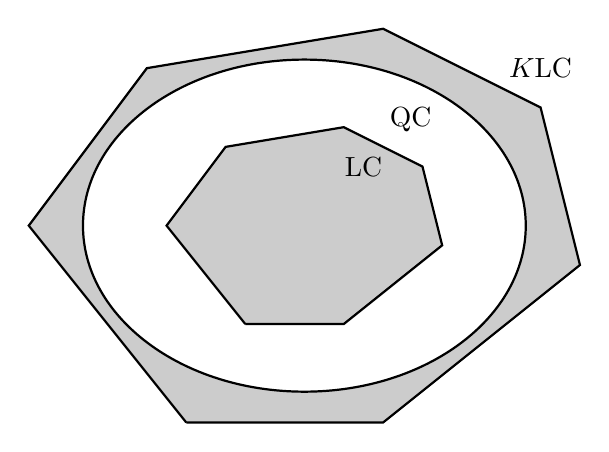
\begin{tikzpicture}[
		-,
		auto,
		node distance=1.6cm,
		thick
	]
	  	\draw[fill=black!20] (-1.5,-2.5) -- (-3.5,0) -- (-2,2) -- (1,2.5) -- (3,1.5) -- (3.5,-.5) -- (1,-2.5) -- (-1.5,-2.5);
	  	\draw[rotate=90, fill=white] (0,0) ellipse (60pt and 80pt);
	  	\draw[fill=black!20] (-0.75,-1.25) -- (-1.75,0) -- (-1,1) -- (0.5,1.25) -- (1.5,0.75) -- (1.75,-0.25) -- (0.5,-1.25) -- (-0.75,-1.25);
	  	\node at (0.75,0.75) {LC};
	  	\node at (1.35,1.35) {QC};
	  	\node at (3,2) {$K$LC};
	\end{tikzpicture}
\end{document}